\begin{bibunit}[IEEEtran.bst]

  \chapter{Modeling and solving altimetry problems}
% \addcontentsline{toc}{chapter}{Modeling and solving altimetry problems}
  \chaptermark{Modeling and solving altimetry problems}
  

This chapter discusses various existing methodologies for modeling and solving tasks related to ocean altimetry. 



Our attention is primarily directed towards techniques that are relevant to the altimetry challenges explored in this study. Most existing methods are geared towards altimetry mapping, as calibration of the Surface Water and Ocean Topography (SWOT) mission is a relatively nascent area with fewer established techniques. Nonetheless, both types of problems aim to estimate the sea surface height $u$ on a domain $\Omega_u$ given observations $y$ on a domain $\Omega_y$.

  Therefore, the methods of interest $f \in \cal{F}$  are such that $f(y) = \hat{u}$ with $\hat{u}$ an estimation of $u$.
   The high level problem can be stated as finding best candidate $\hat(f) \in \mathcal{F}$ using a procedure $c$ that relies on data $\mathcal{D}$. 
   Solving this problem rely on the specification of $\cal{F}$.
  $f$ can be further detailed through the decomposition as $f = f_{x\to u} \circ f_{y\to x}$. The decomposition mainly introduces the choices of intermediate quantities $x$ that characterize the state of an SSH field and a prior distribution $p(x)$. This implies the definition of $f_{x\to u}$ that provides the SSH estimate given a state $x$.
  Secondly, this decomposition implies the choice of a state estimation procedure $f_{y\to x}$ that will determine the state values best suited given observations $y$
$f_{x\to u}$
  Those components fit nicely in the first and second order formulation introduced in the previous chapter as depicted in Figure \ref{c2fig:methodhl}.

\begin{figure}[h]
    \centering
    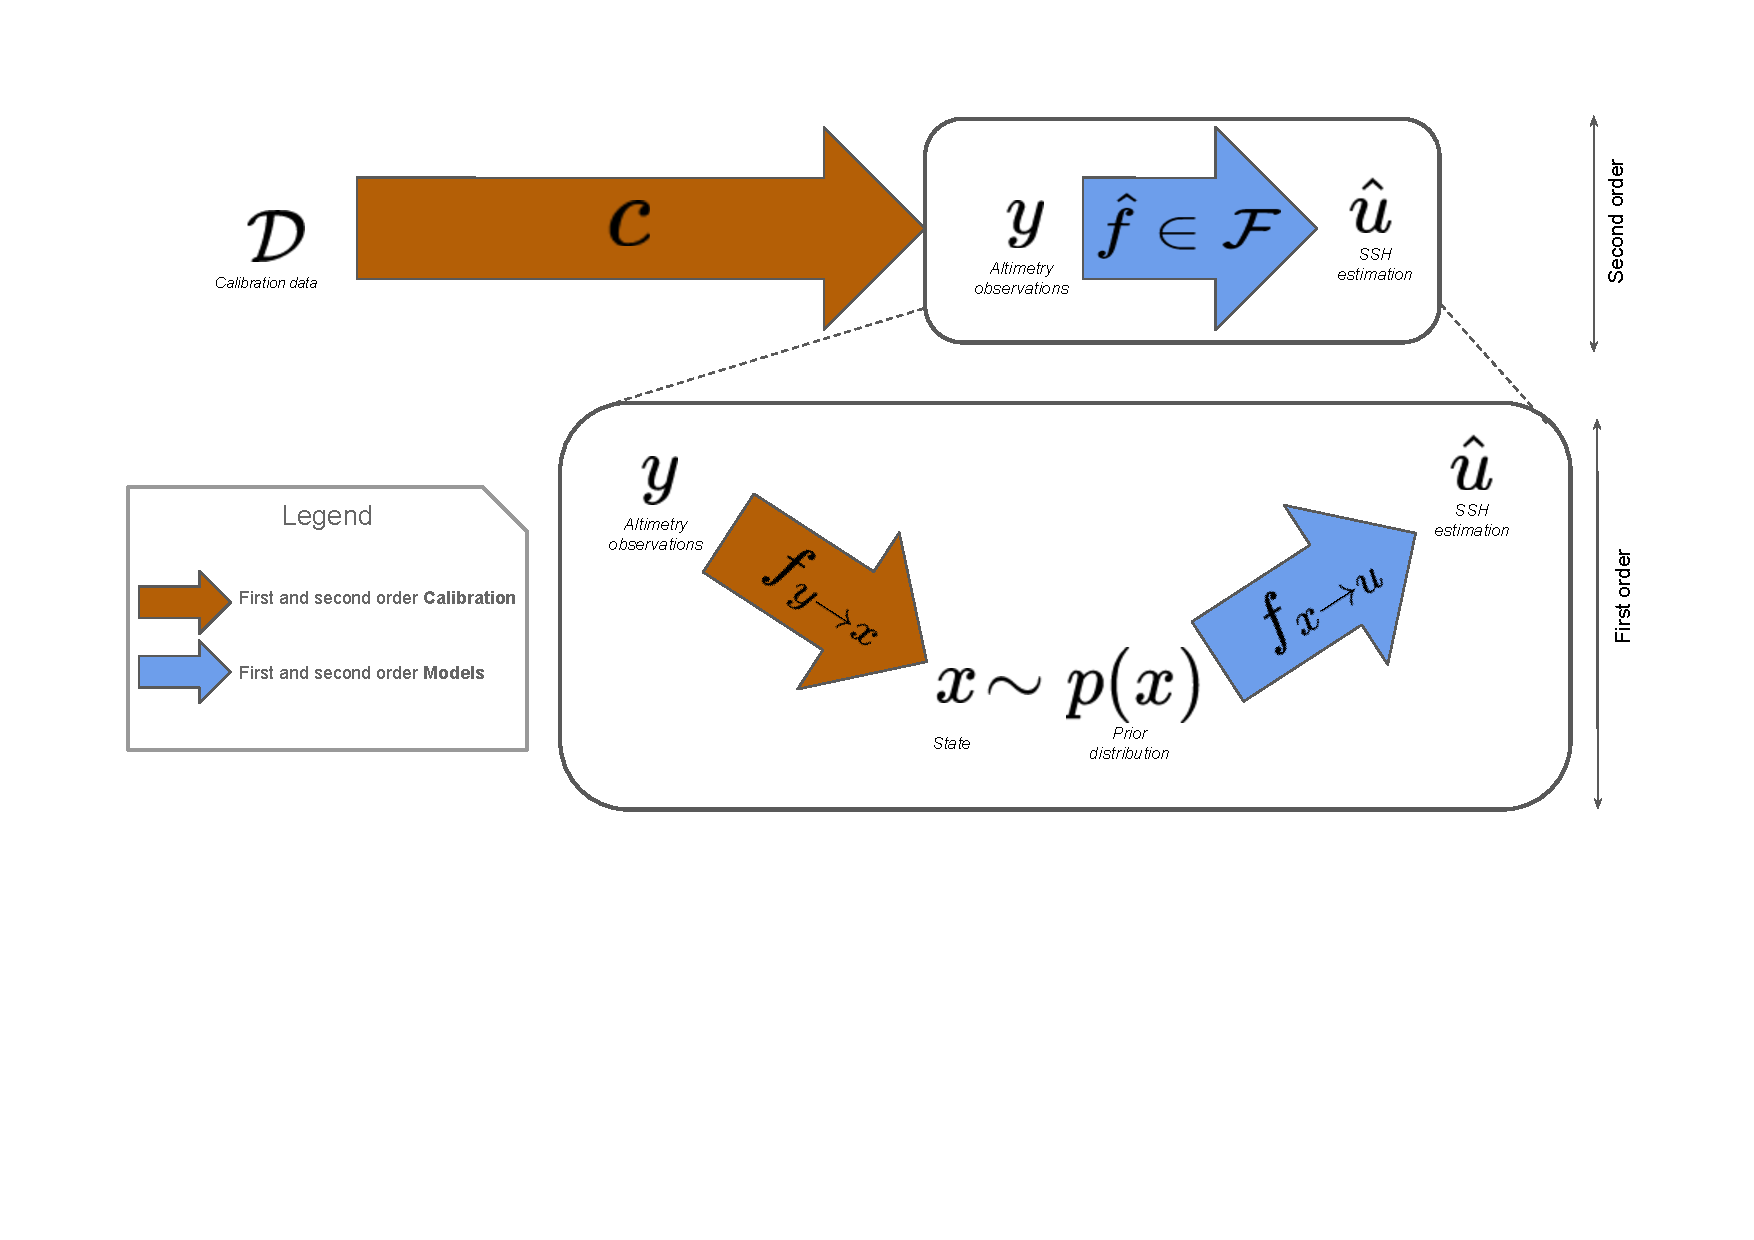
\includegraphics[width=\textwidth, clip,trim=0 5cm 0 0]{00_LitReview/Method-highlevel.pdf}
    \caption{\textbf{Methodological formulation}. This figure illustrate the organization of the different components describe in this chapter}
    \label{c2fig:methodhl}
\end{figure}

  This chapter describes existing approaches for formulating the different components. Possible characterizations of the state $x \tilde p(x)$ are detailed in Section \ref{c2sec:prior} while Section \ref{c2sec:solvers} depicts existing approaches for formulating $f_{y\to x}$. Sections \ref{c2sec:calib} and \ref{c2sec:eval} focus respectively on the calibration $c$ and evaluation considerations.
  The final section \ref{c2sec:4dvarnet} delves into the specific choices of the 4DVarNet framework, which serves as the backbone for the research presented in this thesis.





 \section{Priors on the Sea Surface Height (SSH)}
  \label{c2sec:prior}
The first distinguishing feature among various methods is the choice of characterization of SSH fields. The characterization can be decomposed in two parts.
The first involves the choice of representation $x$ for the target SSH field $u$. This representation essentially outlines the space of all possible SSH states.
The second aims to characterize the probability distribution $p(x)$ of $x$, describing which states are more likely a priori.



 
  \subsection*{State representation}
The choice of state representation defines the quantities $x$ that characterizes the estimated SSH field $\hat{u}$. The choice of $x$ implies the choice of the relationship $\lambda$ between the state values $x$ and the estimated SSH field $\hat{u}$. 


  Looking at existing methods, the SSH field can be characterized through values sampled on a grid or mesh of the domain. These values can directly represent SSH as represented by methods such as the DUACS optimal interpolation \cite{taburetDUACSDT2018252019} (OI), quasi-geostrophic back and forth nudging (BFN-QG) \cite{guillouMappingAltimetryForthcoming2021}, Kalman filtering in GLORYS12 reanalysis \cite{lelloucheCopernicusGlobal122021} or Dynamical Interpolation \cite{ubelmannDynamicInterpolationSea2015,ballarottaDynamicMappingAlongTrack2020} .
  Other methods choose more complex descriptions of the SSH values with large scale and small scale components like in the 4DVarNet\cite{beauchamp4DVarNetSSHEndtoendLearning2023} or even projected values on another basis like MIOST\cite{ubelmannReconstructingOceanSurface2021,ubelmannSimultaneousEstimationOcean2022} which uses a wavelet basis.
  The choices like the mesh, basis or SSH decomposition used is a way to use prior knowledge to dimension the state space. A grid representations of the SSH can be propagated to the whole domain $\Omega_u$ using interpolation schemes which impose additional choices.

  The strong-constraint four dimensional variational data assimilation (s4DVAR)\cite{carrassiDataAssimilationGeosciences2018} consider SSH fields that are solutions to differential equations characterizing the system. The state $x$ then takes the form of initial temporal conditions that are propagated in time using a dynamical model numerical integration scheme. Note that parameters of the model and integration scheme can be part of the state and estimated alongside the initial conditions. 

  Deep learning has introduced new ways of representing the SSH. Notably, Neural fields\cite{johnsonNeuralFieldsFast2022} consists in describing the SSH with the parameters of a coordinate-based neural network. The neural network can then be used to output the SSH value for any given coordinate of the domain.



Finally the state can also contain ancillary quantities that are linked to the SSH. In the GLORYS12\cite{lelloucheCopernicusGlobal122021} reanalysis, the data assimilation scheme considers the state of the ocean beyond the SSH. 
In the case of the SWOT calibration, estimating the SSH is equivalent to estimating the error signals. Operational methods\cite{dibarboureDataDrivenCalibrationAlgorithm2022} approach the problem as defining a state representation of the different error signals.

\subsection*{Prior on the state space}
The representation of SSH $x$ we chose defined the space of all possible states. Additional assumptions can be made to specify which states are more likely than others. This is the prior distribution of the states $p(x)$.
Some approaches like existing work on Neural fields\cite{johnsonNeuralFieldsFast2022} do not define an explicit prior distribution over the state space, which implies a uniform distribution.
Other like OI and s4DVAR shape $p(x)$ through a background state $x_b$ and an error covariance matrix $\mathbf{B}$. Under Gaussian assumptions, the prior distribution becomes 
\begin{equation}
p(\mathbf{x}) = \frac{1}{\sqrt{(2\pi)^n |\mathbf{B}|}} \exp\left(-\frac{1}{2} (\mathbf{x} - x_b)^T \mathbf{B}^{-1} (\mathbf{x} - x_b)\right)
    \label{eq:background}
\end{equation}

In Kalman filters, 3DVAR or weak-constraint four dimensional variational data assimilation (w4DVAR)\cite{carrassiDataAssimilationGeosciences2018}, the likelihood of a state is based on its distance to the trajectory of a dynamical model rather than to a background state giving a similar formulation as above but with $x_b$ replaced by a state-dependent quantity.

Deep learning also introduces tools for probabilistic and energy-based modeling that can be used to characterize $p(x)$.
 For example, 4DVarNet employs a neural network (NN) $\phi$ to define the following quantity over the state space $\| x - \phi(x)\|$. Interpreting this as an energy function, a Boltzmann distribution can be defined the state space, yielding the prior distribution

  \begin{equation}
 p(\mathbf{x}) = \frac{\exp(-\frac{E(\mathbf{x})}{T})}{Z}
    \label{eq:boltzmann}
  \end{equation}
 with $Z = \int \exp(-E(\mathbf{x}) / T) \, d\mathbf{x}$ and $T$ the temperature parameter.



We summarize in the table below the different approaches.
  \begin{table}
  \centering
  \makebox[\textwidth]{
\begin{tabular}{|l|l|l|l|}
\hline
  Method & State formulation & SSH estimation &  Prior formulation\\
\hline
  OI & SSH Grid & Grid Interpolation & Background error \\

  KF, 3DVAR $^{(*)}$ & SSH Grid at time $t$ & Grid Interpolation & Trajectory error \\

  s4DVar & Initial conditions & Trajectory computation & Initial background error \\

  w4DVar & SSH Grid & Grid Interpolation & Trajectory error \\

  MIOST & Wavelet components & Basis change  & Background error \\

  4DVarNet & Scale components & Sum + Grid interpolation  & Energy-based model \\

  Neural field & NN parameters & NN inference & None (Uniform) \\
\hline
\end{tabular}}
\caption{\textbf{Comparison of SSH models across various methods}. The columns indicate the type of state representation $x$, the method of obtaining estimated SSH $\hat{u}$, and the prior distribution $p(x)$. Methods annoted with $^{(*)}$ consider the state of a single time step at a time.}
\end{table}



\section{Solvers: Estimating the state given some observations}
  \label{c2sec:solvers}
Once all prior assumptions about the SSH field have been made (i.e. the first order \textbf{model}), the methods differ by the choice of \textbf{calibration procedure} $f_y{\to x}$. $f_{y\to x}$ defines how to estimate the state $\hat{x}$ given some observations $y$.

This problem can be framed as an inverse problem by defining an observation operator $H$ that describe the relation from state to observations ($f_{y\to x}$ then becomes the inverse $H$).
We define the estimated observations as $\hat{y} = H(x)$. For altimetry observations that measure the quantity of interest $u$, the $H$ operator can be decomposed as $H(x) = f_{x\to u}(x)_{\Omega_y} + \epsilon$ with $\epsilon$ an error term and $f_{x\to u}(x)_{\Omega_y}$ the estimated SSH for a given state $x$ over the observed domain $\Omega_y$. The field of data assimilation in geoscience propose a variety of methods to solve inverse problems.

Using a Bayesian inference formulation, the estimate of the posterior state is done by assuming Gaussian distributions for observation errors and prior states. 
For Optimal Interpolation, this can be mathematically expressed as:
  \begin{equation}
 f_{y\to x}(y)= x_b + K(y - Hx_b)
    \label{eq:KalmanOI}
  \end{equation}
with $H$ a linear observation operator, $x_b$ the background state  and $K$ is the Kalman gain (which depends on $H$, $\mathbf{B}$ and error covariance matrix).
Kalman filters use a similar expression which is applied sequentially for each observation time step.
The procedure $f_{x\to u}$ then becomes a sequence of sub-procedure $f_{x\to u}^1{t1}, ..., f_{x\to u}^{t_n}$ applied to observations $y_{t1}, ..., y_{t_n}$ to estimate the states $x_{t1}, ..., x_{t_n}$ 
  \begin{equation}
f_{y\to x}{t+1}(y_{t+1})= x_{t} + K_{t+1}(y_{t+1} - H_{t+1}M_{t:t+1}x_{t})
    \label{eq:KalmanKF}
  \end{equation}
 with $M_{t:t+1}$ a linear forecast operator and $K_{t+1}$ the kalman gain similarly computed from the error and prediction covariance matrices. 


Variational methods solve the estimation as an optimization problem. The objective is framed as the minimization of a variational cost $\gamma(y) = \arg\min_x J(x, y)$ that includes a observation term $J_{obs}(x, y)$ and a regularization term  $J_{reg}(x)$ related to the prior distribution. The formulation is:

  \begin{equation}
 f_{y\to x}(y) = \arg\min_x \left[ J_{\text{reg}}(x) + J_{\text{obs}}(x, y) \right]
    \label{eq:VarDa}
  \end{equation}
The minimization procedure is classically performed using an iterative gradient based algorithm\cite{carrassiDataAssimilationGeosciences2018}. The gradients can be computed using the adjoint method\cite{lelloucheCopernicusGlobal122021} or automatic differentiation libraries in deep learning\cite{fabletENDTOENDPHYSICSINFORMEDREPRESENTATION2021}.
The calibration of neural fields is also framed as a the minimization of a training objective. However in existing work \cite{johnsonNeuralFieldsFast2022}, since no prior distribution is defined over the states, the variational cost effectively contains only on the observation term.
Such methods are used in variational data assimilation such as 3DVAR, strong and weak 4DVAR, 4DVarNet and can be used to solve the OI problem. Note that similarly to Kalman filters, the 3DVAR method also perform a sequential resolution of the estimation.


Deep learning offers alternative strategies such as direct inversion, where a neural network directly models the function $\gamma$. This eliminates the need for explicitly defining an inverse problem and prior distribution. Example of this approach using classical computer vision models have been applied to altimetry mapping in \cite{manucharyanDeepLearningApproach2021a} and we apply this method in Chapter 3 for SWOT calibration applications.


The different calibration procedures of different methods are summarized in the table below 

\begin{table}
  \centering
  \begin{tabular}{|c|c|c|}
\hline
    Methods & Procedure $f$ \\
\hline
    3DVAR$^{(*)}$, w4DVAR, OI, 4DVarNet & Variational data assimilation \\
    OI, Kalman filters$^{(*)}$ & Bayesian inference \\
    Direct inversion, 4dVarNet & NN inference \\
    Neural fields & Neural network training \\
\hline
\end{tabular}
\caption{\textbf{Comparison of state estimation strategies for existing altimetry methods}. Methods annoted with $^{(*)}$ use a sequential resolution of successive time steps.}
\end{table}

% | Methods    |         estimation         |   O(y, x)   |
% | ---------- |:--------------------------:|:------------:|
% | Nerf       | $\theta = argmin(\cal{L})$ |  $\cal{L}$   |
% | Var        |      $ x = argmin(\alpha R(z) + \beta O(y, x))$      |    $\|y - Hx\|$          |
% | OI, Kalman | $x = x_b + K(y - Hx_b)$ | $\|y - Hx\|$ |
% | Direct Inv |          $x = \phi(y)$          |              |
%




\section{Calibrating the method}
  \label{c2sec:calib}
The choice of prior formulation and estimation procedure provide a method with free parameters (i.e. second order \textbf{model}) that need to be calibrated. 
Calibrating the method involves the fine-tuning of several parameters and model factors. These include the background field, covariance matrices for observation and background errors, as well as specifics for variational optimization or numerical integration schemes. In the case of deep learning approaches like direct inversion, the parameters of the neural network also become factors requiring calibration.


The calibration process relies on datasets, typically comprising numerical model outputs and pre-existing observations. These data sets serve for estimating the aforementioned factors and for validating the performance of the state estimation procedure.
A widely adopted approach for this calibration is cross-validation. In this technique, a subset of available data is utilized to configure the model, which is then tested on the remaining data to evaluate its performance. The exploration of possible configurations may range from manual adjustments to automated parameter tuning algorithms, depending on the complexity of the method being calibrated.

For methods incorporating neural architectures, advanced optimization algorithms specific to deep learning are often employed. These algorithms efficiently tune the weights and biases of the neural network, aligning them for better performance in the SSH estimation task. This is particularly advantageous for direct inversion approaches, which depend entirely on the data for calibration and do not require explicit prior models.

\begin{figure}[h]
    \centering
    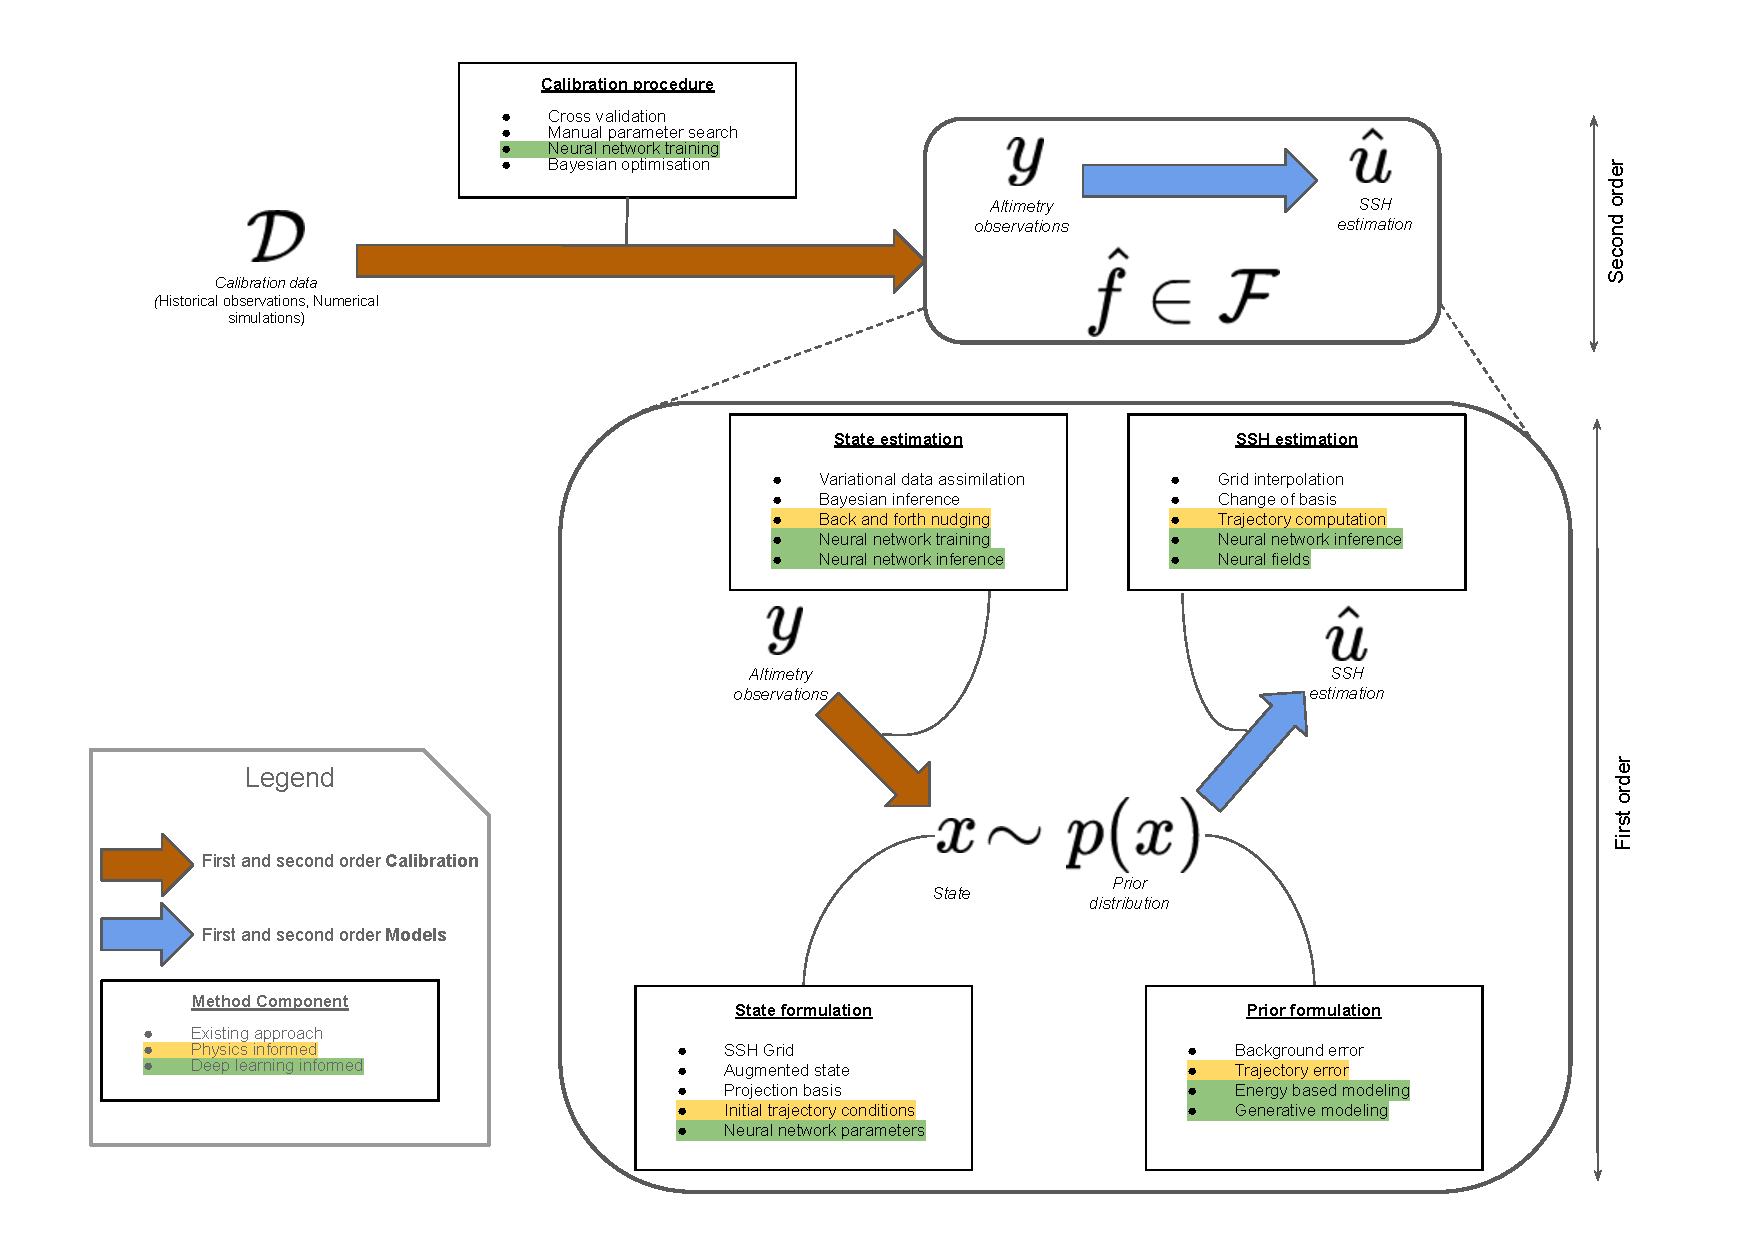
\includegraphics[width=\textwidth]{00_LitReview/Methodology.pdf}
    \caption{\textbf{Solving altimetry problems}. This figure displays the different methodological components in play when addressing an altimetry challenge. The different approaches for each component are detailed and we highlight which ones are physics or deep learning inspired. The specific methods using are detailed below}
    \label{c2fig:method}
\end{figure}


\section{Evaluation}
  \label{c2sec:eval}
So far, we have described the choices made in developing the methods. Yet, a critical choice remains: selecting the criteria to assess the best method for a given problem. To address this, we consider various evaluation data and metrics.

Evaluation data can stem from two main sources, each with its unique risks and benefits. Firstly, the estimated SSH can be compared directly with observation data. Termed as the Observing System Experiment (OSE), its primary advantage lies in its close resemblance to real-world scenarios. However, observational data presents its own challenges. Calibrated nadir altimeters are filtered, unable to capture smaller processes - the same processes anticipated in the new SWOT observations. This poses significant challenges when using nadir altimeter data to assess SWOT calibration. It's worth noting that while data from other observations, such as sea surface temperature or in situ drifter data, can be utilized, they present the challenge of discerning their relationship with the estimated SSH. When mapping altimetry, evaluation using nadir tracks means assessing the SSH over only a portion of the estimated domain. The sampling pattern of nadir altimeters also restricts evaluation. Their sporadic acquisition over time hinders the ability to compare the temporal evolution of the estimation with a reference. Furthermore, the one-dimensional nature of this acquisition precludes the evaluation of pertinent geophysical metrics like the vorticity field.

The second source of evaluation data originates from numerical simulations. Dynamical systems, spanning various complexity levels, can be modeled to produce a 'ground truth' SSH field. Similarly, observing systems can be simulated to produce pseudo-observations. Both types of simulations introduce errors when juxtaposed with real-world scenarios. These errors must be carefully accounted for when interpreting evaluations conducted in such settings. However, this evaluation approach offers considerable flexibility due to the availability of a ground truth.

In this thesis, both scenarios are employed. Chapter 3 examines the SWOT calibration in an OSSE context, while Chapter 4 probes how the evaluation of neural mapping schemes varies between OSSE and OSE contexts.

Several metrics are deliberated upon in this thesis. The primary one is the root mean squared error (RMSE) of the estimated SSH compared to the reference evaluation data. Although this metric provides an easily interpretable value in centimeters, it overlooks some aspects. Since the SSH encompasses processes spanning diverse scales and amplitudes, the normalized RMSE (nRMSE) is also employed to better gauge errors relative to the SSH's amplitude. Specifically, we utilize an nRMSE score $\mu$ defined as $\mu=1 - nRMSE$ (a higher score is preferable). Additionally, oceanic processes of varying amplitudes possess distinctive spatial and temporal scales. The more energetic processes exhibit broader spatial and extended temporal scales. It's imperative for domain experts to ascertain if these processes are aptly depicted in the SSH estimation. Consequently, spectral-based metrics are integral to this thesis. The PSD-score, defined as one minus the ratio of the power spectrum density (PSD) of the error to the reference SSH, is employed. A score closer to one for a given scale indicates minimal error relative to the SSH signal at that scale. Additionally, we define the threshold of spatial scales $\lambda_x$ above which the error signal is below half of the SSH signal. In OSE, $\lambda_x$ calculated along the NADIR altimeter track, while in OSSE, the entire field can be employed. Also, in OSSE, the temporal scales $\lambda_t$ be gauged using the temporal PSD-score.

In closing, a substantial part of assessing an SSH estimation and deciding on pertinent metrics hinges on qualitatively evaluating the field and its temporal evolution, as well as derived geophysical metrics like geostrophic currents and vorticity. Such qualitative evaluations necessitate profound geophysical expertise. Chapter 5 is rooted in these considerations, elucidating and suggesting tools to design appropriate experimental and evaluation frameworks for the adept development and assessment of altimetry mapping methods.



\section{A closer look on the 4dVarNet}
  \label{c2sec:4dvarnet}

\subsection*{Method overview}
The 4dVarNet is a prominent framework frequently employed throughout this thesis which is composed of the following key points.
The SSH field is characterized by values on a regular spatial and temporal grid $x$. The SSH estimate $\hat{u}$ is then obtained using an interpolation scheme $f_{x \to u}$ between the grid points. The prior on the state space is formulated using a neural network $\phi$ as $\|x - \phi(x)\|_{l2}$.
The 4dVarNet framework solves the inverse problem using a variational formulation through the minimization of the cost $J(x, y)$ as stated in  Equation \ref{eq:varcost} 
\begin{equation}
 J(x, y) = \|f_{x\to u}(x)(\Omega_y) - y(\Omega_y)\|_{l2} + \| x - \phi(x)\|_{l2}
    \label{eq:varcost}
  \end{equation}

The minimization procedure consists in an iterative gradient-based method involving a recurrent neural network $\psi$ which is described in Equation \ref{eq:4dinf}.


  \begin{equation}
  \begin{split}
 f_{y\to x}(y) &= \arg\min_x \left[J(x, y) \right] \\
 &= x^N = x^{N-1} - \psi( \nabla_x J(x, y) )
    \label{eq:4dinf}
    \end{split}
  \end{equation}
The calibration of the neural network parameters of $\phi$ and $\psi$ are performed through the end-to-end training scheme on an OSSE dataset $\mathcal{D}$ as put in  Equation \ref{eq:4dtrain}.

  
  \begin{equation}
  \begin{split}
 \hat{f} = \arg\min_f \sum_{(y, u) \in \mathcal{D}} \mathcal{L}(f(y), u)
 \end{split}
    \label{eq:4dtrain}
  \end{equation}


\subsection*{Existing work}
\begin{figure}[h]
    \centering
    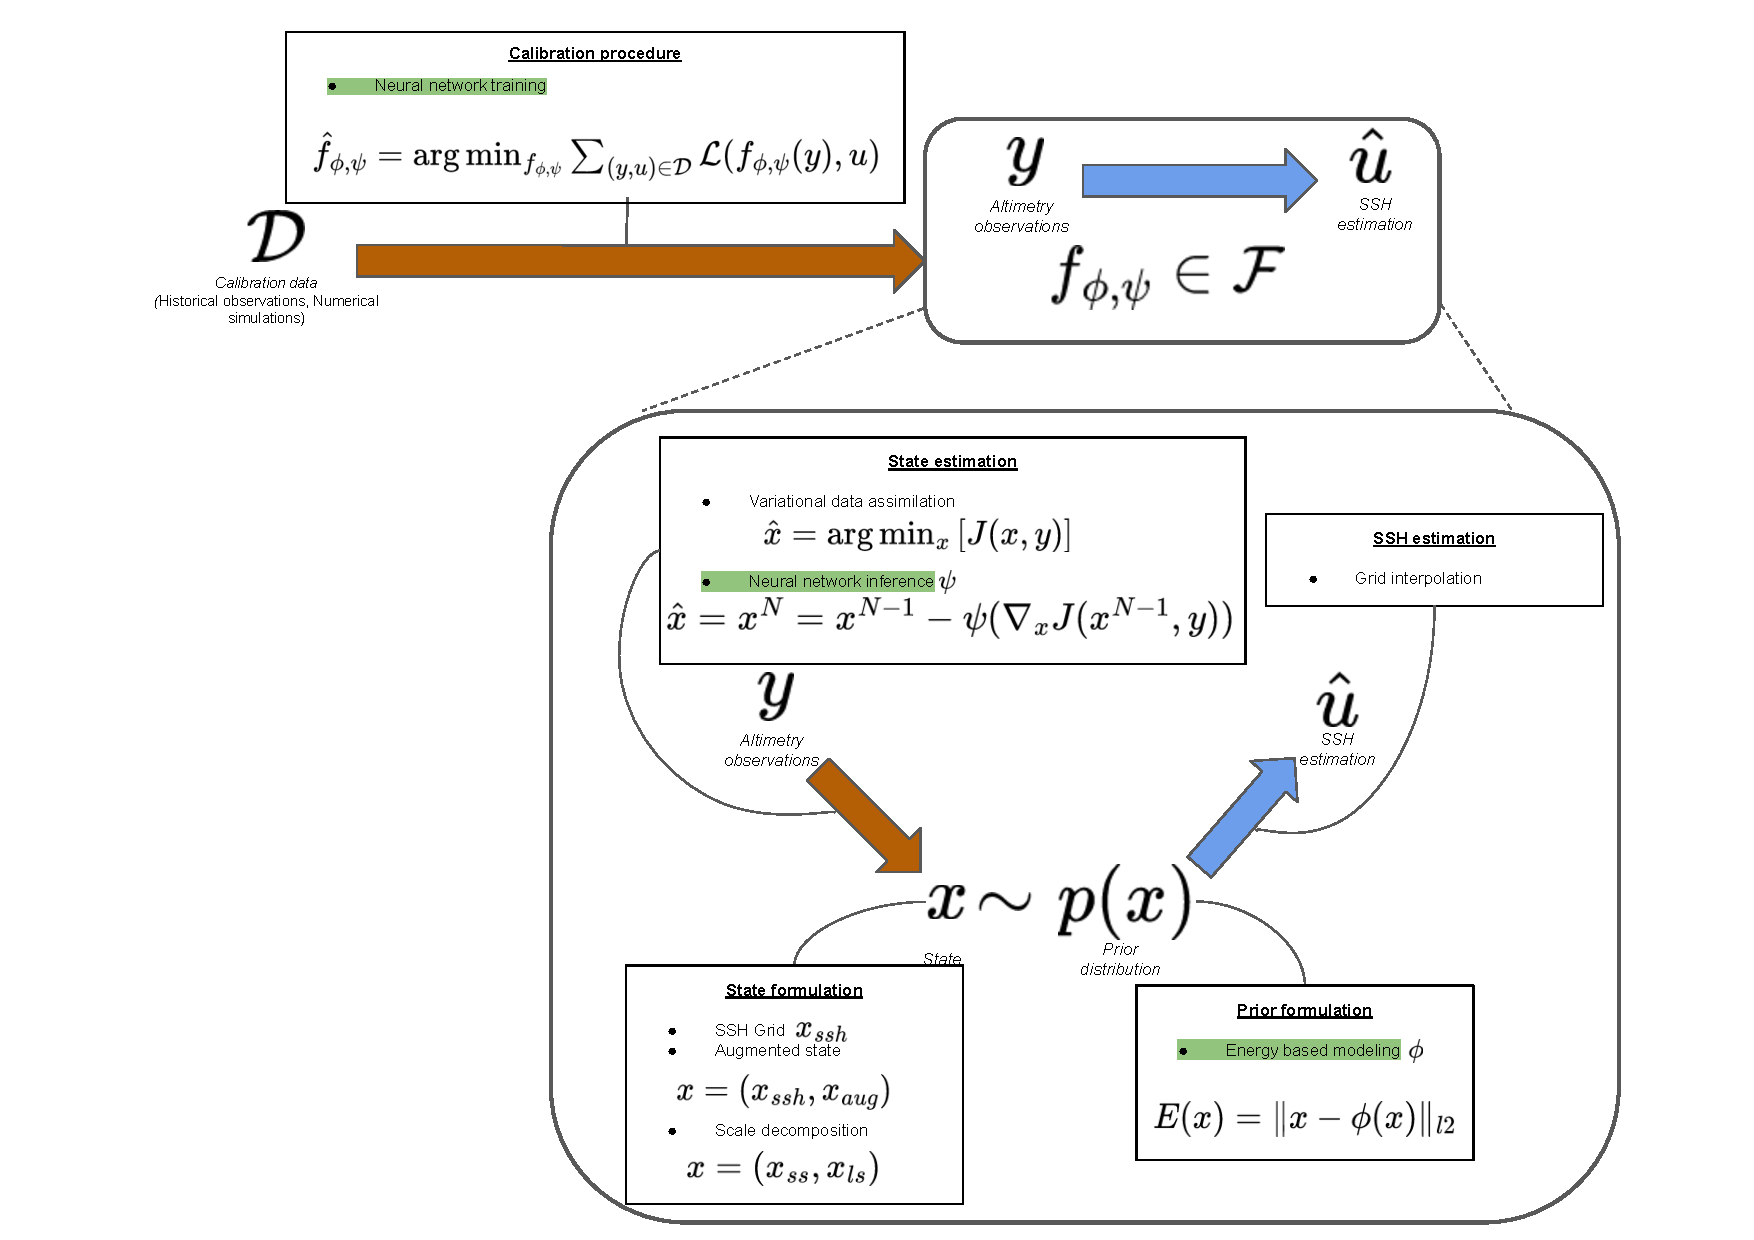
\includegraphics[width=\textwidth]{00_LitReview/Method-4dvarnet.pdf}
    \caption{\textbf{4dVarNet Method components}}
    \label{c2fig:method4}
\end{figure}
In this section, we describe in more detail the different variations of the 4DVarNet in existing work. 
Introduced as a promising approach for mapping altimetry data, 4DVarNet demonstrated robust performance in a study involving simulated SSH based on NATL60 simulation data\cite{fabletENDTOENDPHYSICSINFORMEDREPRESENTATION2021}. Various regions \cite{beauchamp4DVarNetSSHEndtoendLearning2023} and altimetry configurations were considered in these studies, including setups with 4 nadir altimeters both with and without SWOT observations. Earlier versions considered OI-based products as additional observational data for the inversion \cite{fabletENDTOENDPHYSICSINFORMEDREPRESENTATION2021}.

% The representation of the SSH field within the 4DVarNet framework has evolved over time. While earlier studies decomposed SSH into large and small-scale components \cite{beauchampDatadrivenLearningbasedInterpolations2021}, recent implementations used in Chapter 4 represent directly the SSH grid points a single scalar values. In  \cite{fabletENDTOENDPHYSICSINFORMEDREPRESENTATION2021}, latent variables are added to the state to enrich the prior distribution over the state space without being directly constrained by the observations.

The neural network $\phi$ employed for the prior formulation consists in bilinear blocks as introduced in \cite{fabletBilinearResidualNeural2018}. Earlier work \cite{fabletENDTOENDPHYSICSINFORMEDREPRESENTATION2021} used a multiscale architecture while a simpler single scale is used in Chapters 4 and 5. Outside of altimetry, other $\phi$ have been experimented on Lorenz systems including using the true system's dynamics\cite{fabletLearningVariationalData2021}

A Gaussian assumption for the observation errors is commonly adopted, articulated through a quadratic norm in the observation cost. In a study that incorporate Sea Surface Temperature (SST) observations $y_{sst} $\cite{fabletMultimodal4DVarNetsReconstruction2023}, convolutional filters $H_{c1}$, $H_{c2}$ are used to formulate an additional observation cost that relates the state to SST $\| H_{c1}(x) - H_{c2}(y_{sst}\|$.


The neural network $\psi$ is inspired by meta-learning studies \cite{andrychowiczLearningLearnGradient} that employ a Long-Short-Term-Memory (LSTM) to compute state updates\cite{fabletENDTOENDPHYSICSINFORMEDREPRESENTATION2021}. Earlier works used fixed-point algorithms for maximizing observation likelihood, followed by a forward pass using the neural network $\phi$ \cite{beauchampDatadrivenLearningbasedInterpolations2021}. 

Apart from the cross validation and exploration of different architectures and configurations, the training of the neural network's parameters, both for the solver and the prior, is achieved through the Adam optimization algorithm \cite{kingmaAdamMethodStochastic2017}. The aim is to minimize both the mean squared error in SSH reconstruction and its gradients. In order to constrain the estimated states to have low prior costs, a supplementary term is added to ensure effective weightage in the neural prior. This results in the training objective $\mathcal{L}$ described in Equation \ref{eq:loss}.
\begin{equation}
    \mathcal{L}(\hat{u}, u) = \alpha_1\| \hat{u} - u \| 
  + \alpha_2\| \nabla \hat{u} - \nabla u \| 
 + \alpha_3\| \hat{u} - \phi (\hat{u}) \|
 \label{eq:loss}
\end{equation}
4DVarNet has emerged as a versatile and effective architecture for handling altimetry data, with various advancements and optimizations over time. By combining neural networks with traditional variational techniques, it opens up promising avenues for state-of-the-art state estimation in oceanographic applications.

\addcontentsline{toc}{section}{Bibliography}
\putbib[./00_LitReview/LitReview-Biblio.bib]
\end{bibunit}

